
 \documentclass[twocolumn,letterpaper]{igs} 
 
 
\usepackage{lmodern}
\usepackage{amsmath,amssymb,amsthm}
\usepackage{graphicx}
\usepackage{natbib}
\usepackage{wrapfig}
\usepackage{enumitem}
\usepackage{multirow}
\usepackage{tabularx}

\begin{document}

%----------------------------------------------------------------------------------------
%	ARTICLE CONTENTS
%----------------------------------------------------------------------------------------


\section{Methods}

Estimating accumulation from measured values of snow depth and density requires a number of processing steps, each entailing a set of assumptions.  In this study, the steps include (1) measuring snow depth and density, (2) interpolating snow density to estimate snow water equivalent (SWE), (3) averaging measurements within one digital elevation model (DEM) grid cell and (4) interpolating grid-cell SWE values to estimate distributed SWE. To estimate the specific winter surface mass balance (WSMB) we calculate the mean SWE for a grid cell from the estimated distributed SWE. 

\subsection{Measuring snow depth and density}

\begin{figure*}
	\centering
	\includegraphics[width =\textwidth]{Sampling.pdf}\\
	\caption{Sampling design for Glaciers 4, 2 and 13, located in the the Donjek Range, Yukon (a,b). Centreline and transverse transects are shown in blue dots, hourglass and circle design are shown in green dots and zigzag measurements are shown as grey dots (c). Linear and curvilinear transects typically consist of sets of three measurement locations, spaced $\sim$10 m apart (d). At each measurement location, three snow depth observation are made (e). Orange squares are locations of snow density measurements. }
	\label{fig:Sampling}
\end{figure*}

The estimated SWE is the product of the snow depth and density. Snow depth is generally accepted to be more variable than density \citep{Elder1991, Clark2011, Lopez2013} so we chose a sampling design with relatively small measurement spacing along transects that resulted in a ratio of approximately 55:1 snow depth to snow density measurements. The sampling design attempted to capture depth variability at multiple spatial scales and to account for known variation with elevation. Our sampling design is created to avoids bias, allow for the greatest variability to be measured, and minimize distance travelled \citep{Shea2010}.

We measured accumulation at three glaciers to account for range-scale variability \citep{Clark2011}. Snow depth was measured along linear and curvilinear transects to encompass basin-scale variability and at each measurement location, three values of snow depth were recorded to account for point-scale variability \citep{Clark2011}. To exploit the precipitation gradient in the St. Elias Mountains, Yukon \citep{Taylor1969} we measured accumulation on Glaciers 4, 2, and 13 (naming adopted from \cite{Crompton2016}), which are located increasingly far from the head of the Kaskawalsh Glacier (Figure \ref{fig:Sampling}b). We selected centreline and transverse transects with sample spacing of $10-60$ m (Figure \ref{fig:Sampling}d) to capture previously established correlations between elevation and accumulation \citep[e.g.][]{Machguth2006,Walmsley2015} as well as accumulation differences between ice-marginal and center accumulation. We also implemented an hourglass and circle design (Figure \ref{fig:Sampling}), which allows for sampling in all directions and easy travel (Parr, C., 2016 personal communication). At each measurement location, we took $3-4$ depth measurements (Figure \ref{fig:Sampling}e), resulting in more than 9,000 snow depth measurements throughout the study area. 

Our sampling campaign involved four people and occurred between May 5 and 15, 2015, which corresponds to the historical peak accumulation in the Yukon (Yukon Snow Survey Bulletin and Water Supply Forecast, May 1, 2016). While roped-up for glacier travel, the lead person used a hand-held GPS (Garmin GPSMAP 64s) to navigate as close to the predefined transect measurement locations as possible (Figure \ref{fig:Sampling}). The remaining three people used 3.2 m aluminium avalanche probes to take $3-4$ snow depth measurements within $\sim$1 m of each other. Each observer was approximately 10 m behind the person ahead of them along the transect line. The location of each set of depth measurements, taken by the second, third and fourth observer, was approximated based on the recorded location of the first person. 

Snow depth sampling was primarily done in the ablation area to ensure that only snow from the current accumulation season was measured. Determining the boundary between snow and firn in the accumulation area, especially when using an avalanche probe, is difficult and often incorrect \citep{Grunewald2010,Sold2013}. We intended to use a firn corer to extract snow cores in the accumulation area but due to technical issues we were unable to obtain cohesive cores. The recorded accumulation area measurements were done either in a snow pit or with a Federal Sampler so that we could identify the snow-firn transition based on a change in snow crystal size and density. 

When estimating accumulation, snow depth variability at scales less than the grid-size of satellite derived elevation models is assumed to be caused by random effects that are unbiased and unpredictable \citep{Watson2006}. To capture grid-scale variability, we implemented a linear-random sampling design, termed `zigzag' \citep{Shea2010}. We measured depth at random intervals ($0.3 - 3.0$ m) along two `Z'-shaped transects within three to four $40\times40$ m squares (Figure \ref{fig:Sampling}c) aligned with randomly selected DEM grid cells distributed throughout the ablation zone.

Snow density was measured using a wedge cutter in three snowpits on each glacier. We collected a continuous density profile by inserting a $5\times5\times 10$ cm (250 cm$^3$) wedge-shaped cutter in 5 cm increments to extract snow samples and weighed the samples with a spring scale \citep[e.g.][]{Gray1981,Fierz2009}. Uncertainty in estimating density from snow pits stems from measurement errors and incorrect assignment of density to layers that could not be sampled (i.e. ice lenses and `hard' layers). 

While snow pits provide the most accurate measure of snow density, digging and sampling a snow pit is time and labour intensive. Therefore, a Federal Snow Sampler (FS) \citep{Clyde1932}, which measures bulk SWE, was used to augment the spatial extent of density measurements. A minimum of three measurements were taken at $7-19$ locations on each glacier and eight FS measurements were co-located with each snow pit profile. Measurements where the tube snow length was less than 90\% of the snow depth were assumed to be an incorrect sample and were excluded. Density values were then averaged for each location. 

During the field campaign there were two small accumulation events. The first, on May 6, also involved high winds so accumulation could not be determined. The second, on May 10, resulted in 0.01 m w.e accumulation at one location on Glacier 2. High temperatures and clear skies occurred between May 11 and 16, which we believed resulted in significant melt occurring on Glacier 13. The snow in the lower part of the ablation area was isothermal and showed clear signs of melt and snow metamorphosis. Total amount of accumulation and melt during the study period could not be estimated so no corrections were made. 

\subsection{Estimating SWE}

Measured density is interpolated to estimate SWE at each depth sampling location. We chose four separate methods that are commonly applied to interpolate density: (1) mean density over an entire range \citep[e.g.][]{Cullen2017}, (2) mean density for each glacier \citep[e.g.][]{Elder1991, McGrath2015}, (3) linear regression of density with elevation \citep[e.g.][]{Elder1998, Molotch2005} and (4) inverse-distance weighted density \citep[e.g.][]{Molotch2005}. 

When designing the sampling campaign we assumed that SP and FS densities could be combined so that we could have a more spatially distributed density data set. However, there is no correlation between co-located SP and FS densities (Figure \ref{fig:density_pitVStube}). Therefore, SP and FS measurements were used independently for each interpolation method, resulting in eight density interpolation options. 

\subsection{Grid-cell averaging}

We average SWE values within each SPOT-5 DEM-aligned grid cell \citep{Korona2009}. The locations of measurements have considerable uncertainty both from the error of the GPS unit ($2.7 - 4.6$ m) and the estimation of observer location based on the GPS unit. These errors could easily result in the incorrect assigning of a SWE measurement to a certain grid but this source of variability was not further investigated because we assume that SWE variability is captured in the zigzag measurements described below. There are no differences between observers (p$>$0.05), with the exception of the first transect on Glacier 4, so no corrections to the data based on observer are applied.

To encompass variability at spatial scales smaller than a DEM grid cell, we measured snow depth extensively ($135-191$ points) using a `zigzag' configuration (Figure \ref{fig:Sampling}c). Zigzag locations were randomly chosen within the upper ($\sim$2350 m a.s.l.), middle ($\sim$2250 m a.s.l.), and lower portions ($\sim$2150 m a.s.l.) of the ablation area of each glacier. We were able to measure a fourth zigzag on Glacier 13, which was located in the middle ablation area ($\sim$2200 m a.s.l.). SWE variability is assumed to be normally distributed about the mean SWE at a measured grid cell with a standard deviation equal to the average standard deviation of all zigzags on a glacier.

\subsection{Interpolation}

SWE data were interpolated for each glacier using linear regression (LR), simple kriging (SK), as well as regression kriging (RK). Linear regressions relate observed SWE to grid cell values of DEM-derived topographic parameters \citep{Davis1986}. We chose to include elevation, distance from centreline, slope, aspect, curvature, ``northness'' and wind exposure/shelter in the LR. Topographic parameters were weighted by a set of fitted regression coefficients ($\beta_i$). Regression coefficients are calculated by minimizing the sum of squares of the vertical deviations of each data point from the regression line \citep{Davis1986}. The distributed estimate of SWE was found by using regression coefficients to estimate SWE at each grid cell. Specific WSMB was calculated as the mean SWE for each glacier ([m w.e.]). 

The goal of generating a LR is to predict SWE at unsampled grid cells and to tease out dominant relationships between accumulation and topographic parameters. Since snow depth data is highly variable, there is a possibility for the LR to fit to this data noise, a process known as overfitting. To prevent overfitting, cross-validation and model averaging were implemented. Cross-validation was used to obtain a set of $\beta_i$ values that have greater predictive ability. We selected 1000 random subsets (2/3 values) of the data to fit the LR and the remaining data (1/3 values) was used to calculate a root mean squared error (RMSE) \citep{Kohavi1995}. Regression coefficients resulting in the lowest RMSE were selected. Model averaging takes into account uncertainty when selecting predictors and also maximizes predictive ability \citep{Madigan1994}. Models were generated by calculating a set of $\beta_i$ for all possible combinations of predictors. Following a Bayesian framework, model averaging involves weighting all models by their posterior model probabilities \citep{Raftery1997}. To obtain the final regression coefficients, the $\beta_i$ values from each model were weighted according to the relative predictive success of the model, as assessed by the Bayesian Information Criterion (BIC) value \citep{Burnham2004}. BIC penalizes more complex models, which further reduces the risk of overfitting.

Topographic parameters were derived from a SPOT-5 DEM ($40\times40$ km) \citep{Korona2009}. Elevation ($z$) values were taken from the SPOT-5 DEM directly. Distance from centreline ($d_C$) was calculated as the minimum distance between the Easting and Northing of the northwest corner of each grid cell and a manually defined centreline. Slope, aspect and curvature were calculated using the \texttt{r.slope.aspect} module in GRASS GIS software run through QGIS as described in \cite{Mitavsova1993} and \cite{Hofierka2009}. Slope ($m$) is defined as the angle between a plane tangential to the surface (gradient) and the horizontal \citep{Olaya2009}. Aspect ($\alpha$) is the dip direct of the slope and $\sin(\alpha)$, a linear quantity describing a slope as north/south facing, is used in the regression. Mean curvature ($\kappa$) is found by taking the average of profile and tangential curvature. Profile curvature is the curvature in the direction of the surface gradient and it describes the change is slope angle. Tangential curvature represents the curvature in the direction of the contour tangent.Curvature differentiates between mean-concave (positive values) terrain with relative accumulation and mean-convex (negative values) terrain with relative scouring \citep{Olaya2009}. ``Northness'' ($N$) is defined as the product of the cosine of aspect and sine of slope \citep{Molotch2005}. A value of -1 represents a vertical, south facing slope, a value of +1 represents a vertical, north facing slope, and a flat surface yields 0. The wind exposure/shelter parameter (Sx) is based on selecting a cell within a certain angle and distance from the cell of interest that has the greatest upward slope relative to the cell of interest \citep{Winstral2002}. Sx was calculated using an executable obtained from Adam Winstral that follows the procedure outlined in \cite{Winstral2002}. 

Our sampling design ensured that the ranges of topographic parameters covered by the measurements represented more than 70\% of the total area of each glacier (except for the elevation range on Glacier 2, which was 50\%). However, were were not able to sample at locations with extreme parameter values and the distribution of the sampled parameters generally differed from the full distribution.

Visual inspection of the curvature fields calculated using the DEM showed a noisy spatial
distribution that did not vary smoothly. To minimize the effect of noise on parameters sensitive to DEM grid cell size, we applied a $7\times7$ grid cells smoothing window to the DEM, which was then used to calculate curvature, slope, aspect and ``northness''.

Simple kriging (SK) estimates SWE values at unsampled locations by using the isotropic spatial correlation (covariance) of measured SWE to find a set of optimal weights \citep{Davis1986, Li2008}. SK assumes that if sampling points are distributed throughout a surface, the degree of spatial correlation of the observed surface can be determined and the surface can then be interpolated between sampling points. We used the DiceKriging R package \citep{Roustant2012} to calculate the maximum likelihood covariance matrix, as well as range distance and nugget. The range distance is a measure of data correlation length and the nugget is the residual that encompasses sampling-error variance as well as the spatial variance at distances less than the minimum sample spacing \citep{Li2008}. 

Regression kriging (RK) \citep{Hengl2007} estimates were found by first calculating the residuals from the LR estimate at measurement locations. Then, distributed residuals were estimated using SK, and the linear regression SWE and kriged residuals were added to obtain a RK estimate of distributed SWE. Regression kriging can be thought of as an intermediate between pure kriging (no correlation with topographic parameters and large residuals) and pure regression (high correlation with topographic parameters and small residuals) and can be more strongly skewed to either end-member based on the strength of the regression correlation \citep{Hengl2007}.

\subsection{Quantifying effects of variability}

To provide insight on the effects of variability from (1) density interpolation, (2) observed SWE as well as (3) regression estimation on integrated winter surface mass balance, we use a Monte Carlo experiment \citep{Metropolis1949} to estimate a WSMB probability density function (PDF). For all eight density options, normally distributed random variability (mean of zero and standard deviation taken as the mean standard deviation of zigags on a glacier) is introduced to grid-cell values of SWE. LR and SK are used to estimate WSMB and the process is repeated 1000 times.  Variability in regression estimation is accounted for by sampling, with covariance, a multivariate normal distribution of calculated regression coefficients. The covariance of regression coefficients is found according to \cite{Bagos2015}. The process is repeated 1000 times and adjusted $\beta$ values are used to calculate winter surface mass balance. 

%%%%%%%%%%%%%%%%%%%%%%%%%%%%%%%%%%%%%%%%%%
%  RESULTS 
%%%%%%%%%%%%%%%%%%%%%%%%%%%%%%%%%%%%%%%%%%
\section{Results}

\subsection{Measuring snow depth and density}

\begin{figure}
	\centering
	\includegraphics[width =0.5\textwidth]{DepthBoxplot.pdf}\\
	\caption{Boxplot of measured snow depth on Glaciers 4, 2 and 13. The box shows first quartiles, the line within the box indicates data median, bars indicate minimum and maximum values (excluding outliers), and circles show outliers, which are defined as being outside of the range of 1.5 times the quartiles (approximately $\pm2.7\sigma$). }}
	\label{fig:DepthBoxplot}
\end{figure}

A wide range of snow depth is observed on all three study glaciers (Figure \ref{fig:DepthBoxplot}). Glacier 4 has the highest mean snow depth and a high proportion of outliers, indicating a more variable snow depth overall. Glacier 13 has the lowest mean snow depth and a narrower distribution of observed values. At each measurement location, the median range of measured depths ($3-4$ points) as a percent of the mean depth at that location is 2\%, 11\%, and 12\%, for Glaciers 4, 2 and 13, respectively. 

Mean SP and FS density values are within one standard deviation of each other for each glacier and over all three glaciers. The standard deviation of glacier-wide mean density is less than 10\% of the mean density. However, FS densities have a larger range of values ($227-431$kg m$^{-3}$) when compared to SP densities ($299-381$kg m$^{-3}$).  The mean SP densities are within one standard deviation between glaciers, whereas mean FS densities are not.

Uncertainty in SP density is largely due to sampling error of exceptionally dense snow layers. We quantify this uncertainty by varying three values. Ice layer density is varied between 700 and 900 kg m$^{-3}$, ice layer thickness is varied by $\pm$1 cm of the observed thickness, and the density of layers identified as being too hard to sample (but not ice) is varied between 600 and 700 kg m$^{-3}$. The range of integrated density values is always less than 15\% of the reference density, with the largest ranges present on Glacier 2. Density values for shallow pits that contain ice lenses are particularly sensitive to changes in density and ice lens thickness.

\subsection{Estimating SWE}

There is no correlation between co-located SP and FS densities (Figure \ref{fig:density_pitVStube}) so each set of density values is used for all four density interpolation options. Range and glacier mean densities are higher when SP densities are used (Table \ref{tab:Density}). The magnitude and slope of a linear regression of density with elevation differs between SP and FS densities (Table \ref{tab:Density}). At Glaciers 2 and 13, SP density decreases with elevation, likely indicating melt at lower elevations. SP density is independent of elevation on Glacier 4. FS density increases with elevation on Glacier 2 and there is no relationship with elevation on Glaciers 4 and 13. 

There is a positive linear relation (R$^2= 0.59$, p$<$0.01) between measured snow density and depth for all FS measurements. No correlation exists between SP density and elevation.


\begin{figure}
	\centering
	\includegraphics[width =0.5\textwidth]{SPvsFS.pdf}\\
	\caption{Comparison of integrated density estimated using wedge cutters in a snow pit and density estimated using Federal Sampler measurements for Glacier 4 (G04), Glacier 2 (G02) and Glacier 13 (G13). Snow pits were distributed in the accumulation area (ASP), upper ablation area (USP) and lower ablation area (LSP). Error bars are minimum and maximum values.}
	\label{fig:density_pitVStube}
\end{figure}

\begin{table}[]
\centering
\caption{Snow density values used for interpolating density based on snow pit (SP) densities and Federal Sampler (FS) densities. Four interpolation methods are chosen: (1) using a mean snow density for all three glaciers (Range mean density), (2) using a mean density for each glacier (Glacier mean density), (3) using a regression between density and elevation (Elevation regression), and (4) inverse-distance weighted mean density (not shown).}
\label{tab:Density}
\begin{tabular}{cccc}
 &  & \textbf{\begin{tabular}[c]{@{}c@{}}SP density\\ (kg m$^{-3}$)\end{tabular}} & \textbf{\begin{tabular}[c]{@{}c@{}}FS density\\ (kg m$^{-3}$)\end{tabular}} \\
 \midrule
\textbf{\begin{tabular}[c]{@{}c@{}}Range \\ mean density\end{tabular}} &  & 342 & 316 \\
\midrule
\multirow{3}{*}{\textbf{\begin{tabular}[c]{@{}c@{}}Glacier\\ mean density\end{tabular}}} & G4 & 348 & 327 \\
 & G2 & 333 & 326 \\
 & G13 & 349 & 307 \\
 \midrule
\multirow{3}{*}{\textbf{\begin{tabular}[c]{@{}c@{}}Elevation \\ regression\end{tabular}}} & G4 & $0.03z+274$ & $-0.16z+714$ \\
 & G2 & $-0.14z+659$ & $0.24z-282$ \\
 & G13 & $-0.20z+802$ & $0.12z+33$
\end{tabular}
\end{table}

\subsection{Grid-cell averaging}

SWE observations within a DEM grid cell are averaged. Between one and six measurement locations are in each measured grid cell. The distribution of grid-cell SWE values for each glacier is similar to that of Figure \ref{fig:DepthBoxplot} but with fewer outliers. 

SWE measurements for each zigzag are not normally distributed about the mean SWE (Figure \ref{fig:ZigzagHistogram}). The average standard deviation of all zigzags on Glacier 4 is $\sigma_{\mathrm{G4}} =  0.027$ m w.e., on Glacier 2 is $\sigma_{\mathrm{G2}} =  0.035$ m w.e. and on Glacier 13 is $\sigma_{\mathrm{G13}} =  0.040$ m w.e.

\begin{figure}
	\centering
	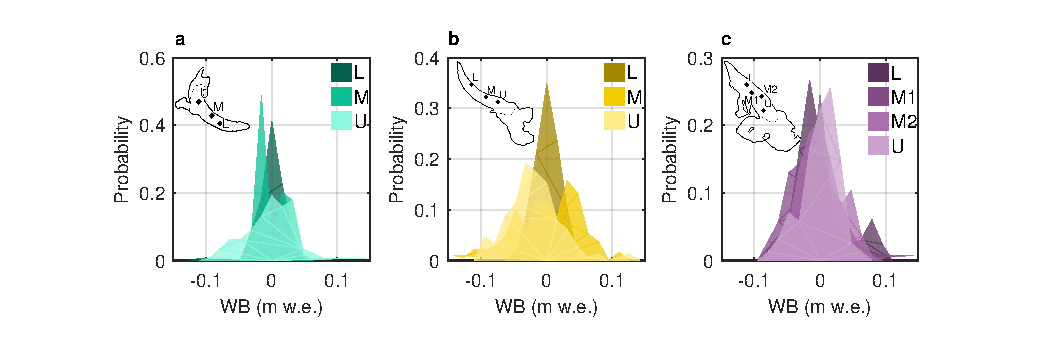
\includegraphics[width =0.5\textwidth]{ZigzagHistogram.pdf}\\
	\caption{Distribution of zigzag SWE values about the local mean on Glacier 4 (upper panel), Glacier 2 (middle panel) and Glacier 13 (lower panel). Zigzags are distributed throughout the ablation area of each glacier, with one located in the lower portion (L), one in the middle portion (M), and one in the upper portion (U). There were two zigzags in the middle ablation area of Glacier 13.}
	\label{fig:ZigzagHistogram}
\end{figure}

\subsection{Interpolation}

The choice of interpolation method affects the mean winter balance (Table \ref{tab:WSMB&RMSE}). SK produces the highest mean WSMB on Glacier 4 and the lowest WSMB on Glacier 13. WSMB estimated by SK is $\sim$30\% lower than WSMB estimated by LR on Glaciers 2 and 13. When using LR, the WSMB on Glaciers 4 and 2 are similar in magnitude.

The predictive ability of SK and LR differ on the study glaciers. Generally, SK is better able to predict SWE at observed grid cells (Figure \ref{fig:observedVSestimated_S2}) and RMSE for all glaciers is lower for SK estimates (Table \ref{tab:WSMB&RMSE}). Glacier 13 has the lowest RMSE regardless of interpolation method, indicating lower SWE variability. The highest RMSE and the lowest correlation between estimated and observed SWE is seen on Glacier 4 (R$^2=$0.12) , which emphasizes the highly variable snow pack.  The highest correlation between estimated and observed SWE is on Glacier 2 when SK is used for interpolation (R$^2=$0.84) (Figure \ref{fig:observedVSestimated_S2}). Residuals for all glacier using LR and SK are normally distributed.

\begin{table}[]
\centering
\caption{Specific winter surface mass balance (WSMB [m w.e.]) estimated using linear regression and simple kriging interpolation for study glaciers. Average root mean squared error (RMSE [m w.e.]) between estimated and observed grid cells that were randomly selected and excluded from interpolation.}
\label{tab:WSMB&RMSE}
\begin{tabular}{ccccc}
 & \multicolumn{2}{c}{\textbf{Linear Regression}} & \multicolumn{2}{c}{\textbf{Simple Kriging}} \\
 & WSMB & RMSE & WSMB & RMSE \\
  \midrule
\textbf{Glacier 4} & 0.582 & 0.153 & 0.616 & 0.134 \\
 \midrule
\textbf{Glacier 2} & 0.577 & 0.102 & 0.367 & 0.073 \\
 \midrule
\textbf{Glacier 13} & 0.381 & 0.080 & 0.271 & 0.068
\end{tabular}
\end{table}

\begin{figure*}
	\centering
	\includegraphics[width =\textwidth]{observedVSestimated_S2.pdf}\\
	\caption{Estimated grid cell SWE found using linear regression (LR) and simple kriging (SK) plotted against observed values of SWE on Glacier 4 (left), Glacier 2 (middle) and Glacier 13 (right). Line of best fit between estimated and observed SWE is also plotted.}
	\label{fig:observedVSestimated_S2}
\end{figure*}

The importance of the various topographic parameters differs for the three study glaciers (Figure \ref{fig:BetaCoeffs}). The most important topographic parameter for Glacier 4 is wind redistribution. However, the wind redistribution coefficient is negative, which indicates less snow in `sheltered' areas. Curvature is also a significant predictor of accumulation where concave areas are more likely to have greater SWE. For Glacier 2, the most important topographic parameter is elevation, which is positively correlated with elevation. Wind redistribution is the second most important topographic parameter and has a positive correlation, which indicates that `sheltered' areas are likely to have high accumulation.The most important topographic parameter for Glacier 13 is elevation. The coefficient is positive, which means that cells at higher elevation had higher values of SWE. Curvature is also a significant topographic parameter but the correlation is negative, indicating less accumulation in convex areas. Most of the topographic parameters are not significant predictors of accumulation on Glacier 13. Aspect and ``northness'' are not significant predictors of accumulation on all study glaciers.

\begin{figure}
	\centering
	\includegraphics[width =0.5\textwidth]{BetaCoeffs.pdf}\\
	\caption{Distribution of regression coefficients for linear regression of grid cell topographic parameters and SWE calculated using eight density options on study glaciers. Topographic parameters include elevation ($z$), distance from centreline ($d_C$), slope ($m$), aspect ($\alpha$), curvature ($\kappa$), ``northness'' ($N$) and wind exposure (Sx). Regression coefficients that were not significant were assigned a value of zero.}
	\label{fig:BetaCoeffs}
\end{figure}

Spatial patterns of SWE found using LR are similar between Glaciers 2 and 13 and differ considerably for Glacier 4. Estimated SWE on Glacier 4 is relatively uniform, which results from the low predictive ability of the LR. Areas with high wind redistribution values (sheltered), especially in the accumulation area, have the lowest values of SWE. The map of modelled SWE on Glacier 2 closely matches that of elevation, which highlights the strong dependence of SWE on elevation. The southwest region of the accumulation area with high estimated accumulation results from the combination of high elevation and Sx values. The low SWE values at the terminus are a result of low elevation values and Sx values that are close to zero. Range of predicted SWE is greatest on Glacier 2 ($0 - 1.92$ m w.e). The map of estimated SWE on Glacier 13 closely follows elevation although the range of SWE values is relatively small so the elevation effect is less pronounced than on Glacier 2.

There are large differences in spatial patterns of estimated WSMB for the three study glaciers found using SK (Figure \ref{fig:LR_SK_map}). Isotropic correlation length is considerably shorter on Glacier 4 (90 m) when compared to Glacier 2 (404 m) and Glacier 13 (444 m), which results in a relatively uniform SWE distribution with small deviations at measured grid cells. Glacier 2 has two distinct and relatively uniform areas. The lower ablation area has low SWE ($\sim$0.1 m w.e.) and the upper ablation and accumulation areas have higher SWE values ($\sim$0.6 m w.e.). Glacier 13 does not appear to have any strong patterns and accumulation is generally low ($\sim0.1-0.5$ m w.e.).

The upper accumulation areas on Glaciers 2 and 13 differ in SWE values when LR and SK are used for interpolation. The significant influence of elevation in the LR results in substantially higher SWE values at high elevation, whereas the accumulation area of the SK estimates approximate the mean observed SWE. 

\begin{figure*}
	\centering
	\includegraphics[width =\textwidth]{LR_map.pdf}\\
    \includegraphics[width =\textwidth]{SK_map.pdf}\\
	\caption{Spatial distribution of SWE estimated using linear regression (upper) and simple kriging (lower). Grid-cell SWE observations are calculated using glacier wide mean snow pit density and are shown as black dots. Glacier flow directions are indicated by arrows. Specific WSMB values are also shown.}
	\label{fig:LR_SK_map}
\end{figure*}

Transferring LR coefficients between glaciers results in a high range scale mean RMSE. The lowest RMSE (0.2051 m w.e.) results from calculating a LR using all available observations. Elevation is the only significant topographic predictor for a range-scale LR ($\beta_z=0.0525$).


\subsection{Quantifying effects of variability}

Specific winter surface mass balance (WSMB) is affected by variability introduced when interpolating density, estimating grid cell SWE values, and when interpolating observations. When using a LR, variability in estimating regression coefficients has a larger effect on WSMB uncertainty than density interpolation variability or grid cell SWE variability. The probability density function (PDF) for SWE variability is much narrower than that for regression coefficient variability (Figure \ref{fig:WSMBDist_LR} and Table \ref{tab:WSMBdistribution_sigma}). SK interpolation uncertainty is dominated by density interpolation variability on Glaciers 4 and 13 but by SWE variability on Glacier 2 (Table \ref{tab:WSMBdistribution_sigma}). 

 \begin{table}[]
\centering
\caption{Mean standard deviation ([m w.e.]) of specific winter surface mass balance estimated using linear regression and simple kriging when variability is introduced. Variability in grid cell SWE is approximated by a normal distribution about the local SWE value with standard deviation equal to the glacier-wide mean zigzag standard deviation ($\sigma_{ZZ}$). Variability in regression estimation is accounted for by varying the regression coefficients with a normal distribution with standard deviation calculated from regression covariance ($sigma_{\beta}$).}
\label{tab:WSMBdistribution_sigma}
\begin{tabular}{ccccccc}
 & \multicolumn{4}{c}{\textbf{Linear Regression}} & \multicolumn{2}{c}{\textbf{Simple Kriging}} \\
 & $\rho$ & $\sigma_{ZZ}$ & $sigma_{\beta}$ & $\sigma_{ZZ}$ \& $\sigma_{\beta}$ & $\rho$ & $\sigma_{ZZ}$ \\
\textbf{Glacier 4} & 0.0204 & 0.0086 & 0.0213 & 0.0231 & 0.0202 & 0.0086 \\
\textbf{Glacier 2} & 0.0263 & 0.0180 & 0.0309 & 0.0377 & 0.0187 & 0.0256 \\
\textbf{Glacier 13} & 0.0112 & 0.0112 & 0.0232 & 0.0280 & 0.0138 & 0.0116
\end{tabular}
\end{table}

\begin{figure*}
	\centering
	\includegraphics[width =\textwidth]{WSMBDist_LR.pdf}\\
	\caption{Probability density functions (PDFs) fitted to distributions of specific winter surface mass balance (WSMB) values that arise from SWE variability ($\sigma_{ZZ}$) and regression estimation ($\sigma_{\beta}$). Each PDF is calculated using one of eight density interpolation methods for Glacier 4 (G4), Glacier 2 (G2) and Glacier 13 (G13).}
	\label{fig:WSMBDist_LR}
\end{figure*}

The full WSMB uncertainty PDF when LR or SK is used for interpolation differs significantly on Glaciers 2 and 13. With a LR interpolation, the PDF for Glaciers 4 and 2 completely overlap, while the PDF of Glacier 13 is centred at a lower WSMB. However, SK interpolation results in three distinct PDFs, with the PDFs of Glaciers 2 and 13 centred at lower WSMB values. 

\begin{figure*}
	\centering
	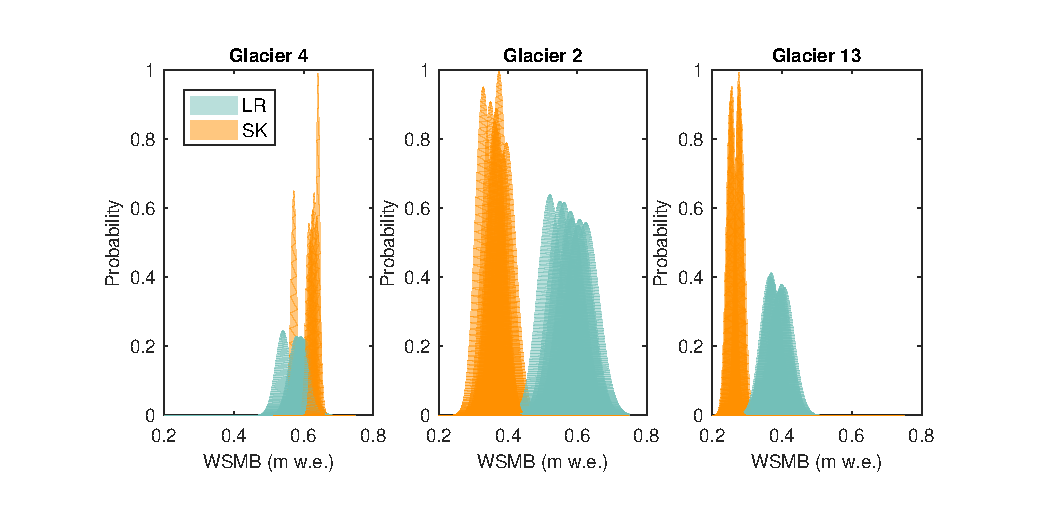
\includegraphics[width =\textwidth]{WSMBDist_LRvsSK.pdf}\\
	\caption{Probability density functions (PDFs) fitted to distributions of specific winter surface mass balance (WSMB) values estimated using linear regression (LR) or simple kriging (SK). Each PDF is calculated using one of eight density interpolation methods for Glacier 4 (left), Glacier 2 (middle) and Glacier 13 (right).}
	\label{fig:WSMBDist_LRvsSK}
\end{figure*}

\begin{figure*}
	\centering
	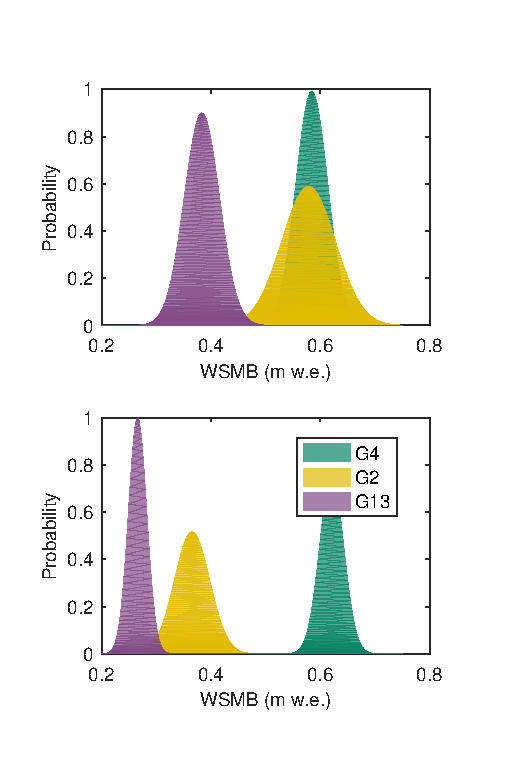
\includegraphics[width =\textwidth]{WSMBDist_full.pdf}\\
	\caption{Probability density functions (PDFs) fitted to distributions of specific winter surface mass balance (WSMB) values estimated using linear regression (top) or simple kriging (bottom). Each PDF includes density variability, SWE variability and regression estimation (linear regression only) for Glacier 4 (G4), Glacier 2 (G2) and Glacier 13 (G13).}
	\label{fig:WSMBDist_LRvsSK}
\end{figure*}


The spatial patterns of WSMB are affected by density, SWE, and regression variability (Figure \ref{fig:WSMBspatialvar}).  For both LR and SK, the greatest variability in estimated SWE occurs in the accumulation area. When LR is used, estimated SWE is highly sensitive to the elevation regression parameter. In the case of SK, variability is greatest in areas far from observed SWE, which consist of the upper accumulation area on Glaciers 2 and 13. On Glacier 4, variability is greatest at the upper edges of the accumulation area, which corresponds to the locations with extreme values of wind redistribution parameter. When SK is used for interpolation on Glacier 4, variability is greatest at the measured grid cells, which highlights the short correlation length and the large effect of density interpolation on the SK accumulation estimate.

\begin{figure*}
	\centering
	\includegraphics[width =\textwidth]{SpatialVar_LR.pdf}\\
	\includegraphics[width =\textwidth]{SpatialVar_SK.pdf}\\
	\caption{Variability of SWE estimated using linear regression (top) and simple kriging (bottom).	Variability is measured by taking the sum of differences between one hundred estimates of distributed WSMB that include SWE variability and, in the case of linear regression, regression variability. The sum is then normalized for each glacier.}
	\label{fig:WSMBspatialvar}
\end{figure*}



%------------------------------------------------

\section{Discussion}
[77] conducted an airborne GRP survey of two adjacent glaciers in Switzerland. The
lower part of the larger valley glacier showed a clear correlation between altitude and snow
accumulation. The upper part of the glacier and the adjacent smaller glacier had no alti-
tudinal trend and the fluctuations in depth were large. Additionally, the accumulation was
40\% lower on the smaller glacier. The altitudinal trend is a well documented pattern and
was thought to be a result of melt that occurred during warmer weather, which is more
pronounced at lower elevations. Spatial variability of precipitation and redistribution of
snow were believed to have resulted in the high spatial variability in higher parts of the
study area. Since the majority of the precipitation events originated from one direction and
the large glacier was on the lee side of a ridge, it experienced preferential deposition. Mean-
while, the smaller glacier was further along the storm track so it received less precipitation.
Overall, [77] showed that snow distribution on glaciers is not simply a function of altitude,
which corroborated research done in other alpine catchments.

 In most cases, the resolution of measurements over a large area is insufficient to
approximate the true variability [15, 32].


 The estimates of SWE in the accumulation area are greatest when kriging is used because there is a single single high SWE value in the accumulation area. Kriging is sensitive to outliers in areas with sparse sampling. Kriging estimates lower SWE in the accumulation area of both glaciers because elevation is not incorporated into the model.

extrapolation of regression models will
likely result in large errors. These errors are especially relevant in the accumulation area,
which has extreme values for all parameters. Errors in the accumulation area are especially
important to acknowledge because this area has the highest values of SWE and is likely to
heavily influence final winter mass balance values. Improvements to this study could include
using an air-borne GPR to collect a dense network of SWE measurements in difficult to
access areas [e.g. 82] (see Section 1.3.2 for more details).


 and both under and over sampling is believed to have occurred using the FS (more details or just sources??). 


Lopez 2013 for small scale var

Winter snow pack in southwestern Yukon was well below normal in 2015 (Yukon Snow Survey Bulletin and Water Supply Forecast, May 1, 2016). Temperatures were generally warmer than normal and the melt season began $1-2$ weeks early. 

Field sampling (also called direct glaciological method) is known to be biased towards small alpine glaciers with simple topography.

The Sx coefficient is negative, which indicates less snow in ‘sheltered’ areas. The negative correlation is counter intuitive so it is surprising that Sx is the best predictor for accumulation.
 Areas with high Sx values (sheltered), especially in the accumulation area, have the lowest values of SWE. This regression indicates that the wind plays a role in snow distribution but since the valley in which the glacier sits is steep walled and curved, perhaps having a single cardinal direction for wind is inappropriate. Examining Sx values that assume wind moving up or down glacier and changing direction to follow the valley could allow the Sx parameter to explain more of the variance.





The range of predicted SWE is largest for Glacier 2 and it also has the highest SWE (1.92 m w.e) and the lowest SWE (0 m w.e.) values. Both extremes are perhaps unexpected on this glacier and are likely an artefact from extrapolating from the regression, which largely depends on elevation.







\section{Introduction}

Objective: (1) Discuss choices made when moving from measurement to accumulation and (2) show how system variability and our choices interact to create uncertainty in our estimate of accumulation

- snow distribution in alpine regions is not uniform or static, but
rather highly variable and influenced by diverse and dynamic processes operating on multiple spatial and temporal scales -> topographic effects (crevasses, surface topo, elevation aspect, precip grad across range), snow drift and preferential deposition
-  [22] note that studies of snow water equivalent (SWE) that have been conducted in
alpine environments vary considerably in the extent and spacing of their measurements.
- Snow accumulation is spatially variable on point scales (<5 m), hillslope scales (1–100 m),
basin scales (100–10,000 m) and regional scales (10–1000 km) [22].
-Point-scale variability is generally associated with surface roughness effects and the
presence of small obstacles. -> take three measures
Many parts of a glacier though
are characterized by a relatively smooth surface, with roughness lengths on the order of
centimeters [57]. In these areas, point-scale variability of snow depth is low. However, in
heavily crevassed regions, point-scale variability can be large and thus exert a dominant
control on snow distribution in the area [82].
-Hillslope-scale variability is caused by variations in the surface topography of the glacier.
The curvature and slope of the surface as well as the presence of local ridges or depressions
can affect where snow is located [15, 115]. Avalanching can also redistribute snow, especially
on the margins of a glacier [17, 89].
Watershed-scale variability results mainly from the effects of changing elevation and
aspect on atmopsheric conditions [22]. In particular, orographic lifting and shading can
result in higher elevation and north-facing areas of the glacier having more snow than other
areas [89, 115]. Gradients in temperature from elevation changes also affect the freezing
level, which determines whether precipitation falls as snow or rain [17]. For example, [77]
found a strong influence of elevation in determining accumulation on Findel Glacier in
Switzerland.
Regional variability occurs when areas within a mountain range have differing amounts of
snow. Often, this results from horizontal precipitation gradients and rain shadows forming
on the lee side of topographic divides. Areas with large, steep mountains are especially
affected by these processes.

----------------------------------------------------

derived accumulation
estimated winter surface mass balance
distributed snow water equivalent
%------------------------------------------------



%----------------------------------------------------------------------------------------
%	REFERENCE LIST
%----------------------------------------------------------------------------------------

\bibliography{/home/glaciology1/Documents/MastersDocuments/MastersLit}
\bibliographystyle{igs}

%----------------------------------------------------------------------------------------

\end{document}
